\section{Příklad 2}
% Jako parametr zadejte skupinu (A-H)
\druhyZadani{C}

\begin{center}
    \begin{LARGE}
        Řešení metodou Théveninovy věty
    \end{LARGE}
\end{center}
\setcounter{figure}{0}

% Krok 1
\begin{itemize}
    \item Zjednodušíme $R_4$, $R_5$ (sériové zapojení) a odstraníme odpor $R_3$, zdroj napětí $U$
\end{itemize}

\begin{figure}[h]
    \centering
    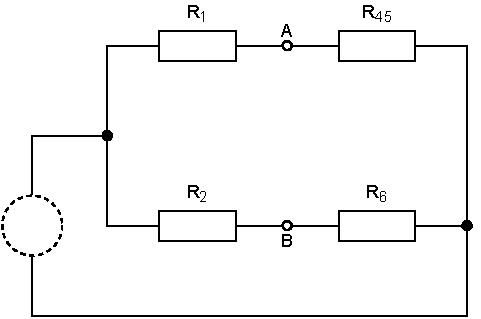
\includegraphics[scale=0.8,keepaspectratio]{fig/Pr2_krok1.pdf}
    \caption{Upravený obvod}
    \label{pic:Pr2_krok1}
\end{figure}

\begin{center}
    \begin{gather*}
        R_{45} = R_4 + R_5 = 240 + 450 = 690 \: \Omega \\
    \end{gather*}
\end{center}

\newpage

% Krok 2
\begin{itemize}
    \item Najdeme $R_{145}$ a $R_{26}$ (paralelní zapojení), pak spočítamé $R_i$ (sériové zapojení)
\end{itemize}

\begin{figure}[h]
    \centering
    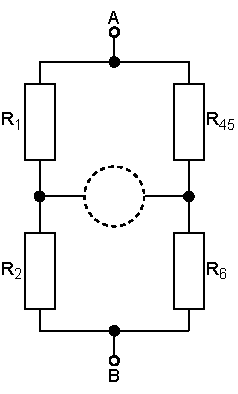
\includegraphics[scale=0.8,keepaspectratio]{fig/Pr2_krok2_1.pdf}
    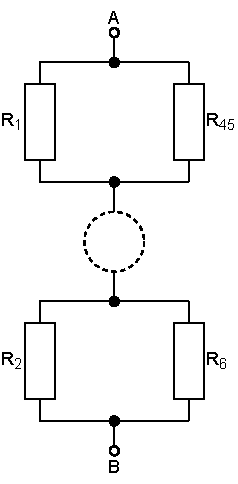
\includegraphics[scale=0.8,keepaspectratio]{fig/Pr2_krok2_2.pdf}
    \caption{Výpočet $R_i$}
    \label{pic:Pr2_krok2}
\end{figure}

\begin{center}
    \begin{gather*}
        R_{145} = \frac{R_1 \times R_45}{R_1 + R_{45}} = \frac{70 \times 690}{70 + 690} = 63,5526 \: \Omega \\[6pt]
        R_{26} = \frac{R_2 \times R_6}{R_1 + R_{45}} = \frac{220 \times 300}{220 + 300} = 126,9231 \: \Omega \\[6pt]
        R_i = R_{145} + R_{26} = 63,5526 + 126,9231 = 190,4847 \: \Omega \\
    \end{gather*}
\end{center}

\newpage

% Krok 3
\begin{itemize}
    \item Spočítáme $U_{R_1}$, $U_{R_2}$ při pomoci napěťového děliče a určíme $U_i$
\end{itemize}

\begin{figure}[h]
    \centering
    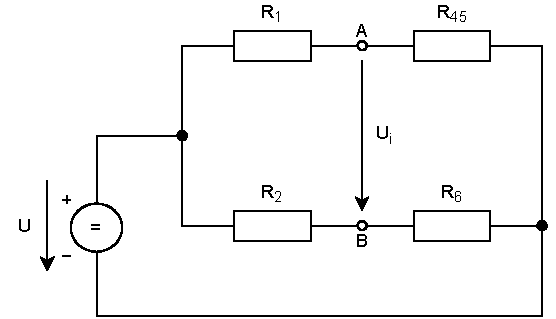
\includegraphics[scale=0.8,keepaspectratio]{fig/Pr2_krok3.pdf}
    \caption{Výpočet $U_i$}
    \label{pic:Pr2_krok3}
\end{figure}

\begin{center}
    \begin{gather*}
        U_{R_1} = U \times \frac{R_1}{R_1 + R_{45}} = 200 \times \frac{70}{70+690} = 18,4211 \: V \\[6pt]
        U_{R_2} = U \times \frac{R_2}{R_2 + R_6} = 200 \times \frac{220}{220+300} = 84,6154 \: V \\[6pt]
        U_i = U_{R_2} - U_{R_1} = 84,6154 - 18,4211 = 66,1943 \: V \\
    \end{gather*}
\end{center}

% Krok 4
\begin{itemize}
    \item Spočítáme $I_{R_3}$ a $U_{R_3}$ (Ohmův zákon)
\end{itemize}

\begin{figure}[h]
    \centering
    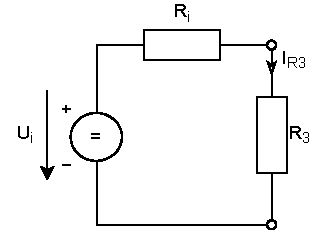
\includegraphics[scale=0.8,keepaspectratio]{fig/Pr2_krok4.pdf}
    \caption{Výpočet $I_{R_3}$ a $U_{R_3}$}
    \label{pic:Pr2_krok4}
\end{figure}

\begin{center}
    \begin{gather*}
        I_{R_3} = \frac{U_i}{R_i + R_3} = \frac{66,1943}{190,4847+630} = 0,0807 \: A \\[6pt]
        U_{R_3} = I_{R_3} \times R_3 = \frac{66,1943}{190,4847+630} \times 630 = 50,8266 \: V
    \end{gather*}
\end{center}